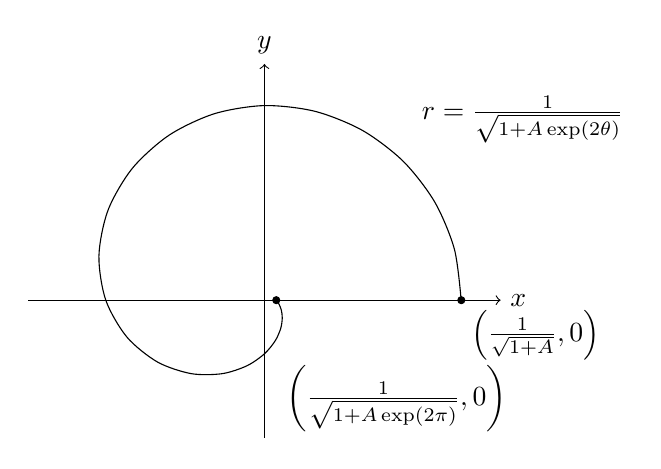
\begin{tikzpicture}[scale=2.5]
    \draw[->] (-1.2, 0) -- (1.2, 0) node[right] {\(x\)};
    \draw[->] (0, -0.7) -- (0, 1.2) node[above] {\(y\)};

    \draw[color=black, domain=0:2*pi, smooth] plot ({\x r}:{1/sqrt(1+0.001*exp(2*pi)*exp(2*(\x-pi)))}) node at (0.75, 0.75) [above right] {\(r = \frac{1}{\sqrt{1 + A \exp(2\theta)}}\)};

    \draw[fill=black] (1, 0) circle (0.5pt) node [below right] {\(\left(\frac{1}{\sqrt{1 + A}}, 0\right)\)};
    \draw[fill=black] (0.06, 0) circle (0.5pt) node [below right, yshift=-20pt] {\(\left(\frac{1}{\sqrt{1 + A \exp(2\pi)}}, 0\right)\)};
\end{tikzpicture}